\chapter{Introduksjon}
%--------------------MÅ INN I HOVEDRAPPORT------------------------------------------
Rotårsaksanalyser er et lite brukt verktøy innen informasjonssikkerhet, men er av økende betydning. Vanlig tilnærming til informasjonssikkerhetsstyring er å utføre en risiko-og sårbarhetsanalyse (ROS-analyse) for så å gjennomføre tiltak som fører risikoene til et akseptabelt nivå. En annen hyppig brukt tilnærming er hendelseshåndtering der en planlegger hvordan det skal responderes på hendelser etter de er inntruffet. Rotårsaksanalyse skiller seg fra disse ved å gå i dybden på problemet, kartlegge hva slags rotårsaker som står bak, og innføre tiltak for å fjerne disse helt.
%%%%%%%%%%%%%%%%%%%%%%%%%%%%%%%%%%%%%%%%%%%%%%%%%%%%%%%%%%%%%%%%%%%%%%%%%%%%%%%%%%%%%

\section{Oppgavebeskrivelse}
Denne rapporten er en delrapport i en større oppgave om rotårsaksanalyse. Dette caset går inn på rotårsaken til at brukere på skolenettet til NTNU laster ned opphavsrettsbeskyttet materiale.

Hver måned får NTNU ca. 150 og 200 unike notifikasjoner om brudd på opphavsretten ved ulovlig fildeling. Vi kan se at dette nummeret går kraftig ned i sommermånedene, som tilsier at studentene er hovedgrunnen til bruddene på opphavsrett. Se \hyperref[fig:copyright]{Figur 1} under for en grafisk illustrasjon av antall notifikasjoner for brudd på opphavsrett.

\begin{figure}[H]
    \centering
    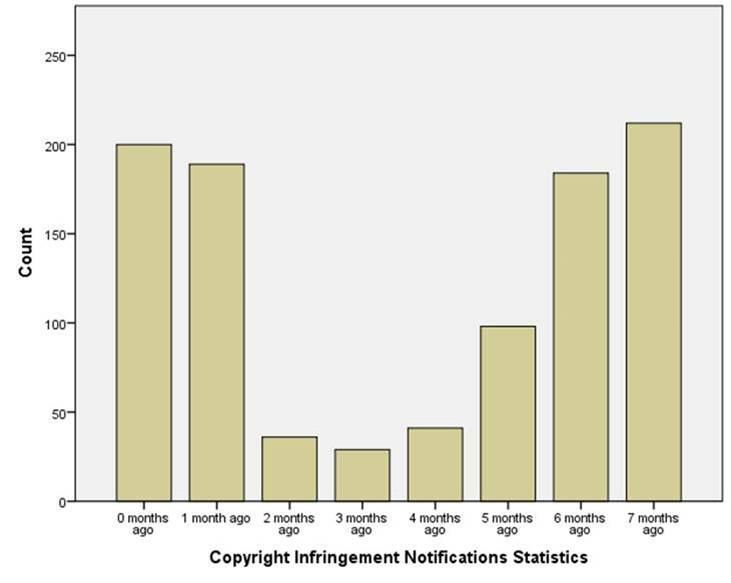
\includegraphics[scale=0.8]{copyright}
    \label{fig:copyright}
    \caption[Copyright Infringement Notifications]{Copyright Infringement Notifications}
\end{figure}

\begin{comment}
\begin{table} [H]
    \begin{tabular}{ | m{12em} | m{12em} | m{12em} | }
        \hline
            \cellcolor{yellow} & \cellcolor{yellow} Breaches & \cellcolor{yellow} Copyright breach/Piracy\\
        \hline
            Policy Violation & Information Security Policy & 2 \\
        \hline
             & IT Policy & 43 \\
        \hline
    \end{tabular}
    \caption{Oversikt over kvantiteten av brudd på policy}
    \label{kritisk_tabell_1}
\end{table}
\end{comment}

For å utrede problemstillingen basert på informasjonen over, er følgende forskningsspørsmål valgt: 
\begin{itemize}
    \item Hva er rotårsaken til at studenter laster ned opphavsrettsbeskyttet materiale?
    \item Hvordan fungerer rotårsaksanalyse i et case som omhandler ulovlig fildeling?
\end{itemize}

Å få svar på dette, ikke nødvendigvis i tilknytning til NTNU's nettverk, kan også være nyttig for videre arbeid.

Når vi i denne rapporten bruker ordet fildeling, omtaler vi fildeling ved bruk av torrents. Annen fildeling går ikke under vårt bruk av begrepet og heller ikke under problemstillingen. Begrepet torrents brukes fortsatt når vi snakker om selve teknologien og sporingen av de enkelte torrentene.

I oppgaven avgrenser vi oss til NTNU Gjøvik, og ser bare på nettverket til de ulike studentbyene tilknyttet SIT Bolig. Nettet på campus faller ikke under problemstillingen.

\section{Metode}
Metodebruken i denne analysen er delt inn i syv steg som vist i \hyperref[fig:prosess]{Figur 2} under. I hvert steg av denne prosessen brukes det ulike verktøy for å hjelpe til med å forstå problemet, finne rotårsak, og tilslutt implementere tiltak for å eliminere årsakene. 
\begin{figure}[H]
    \centering
    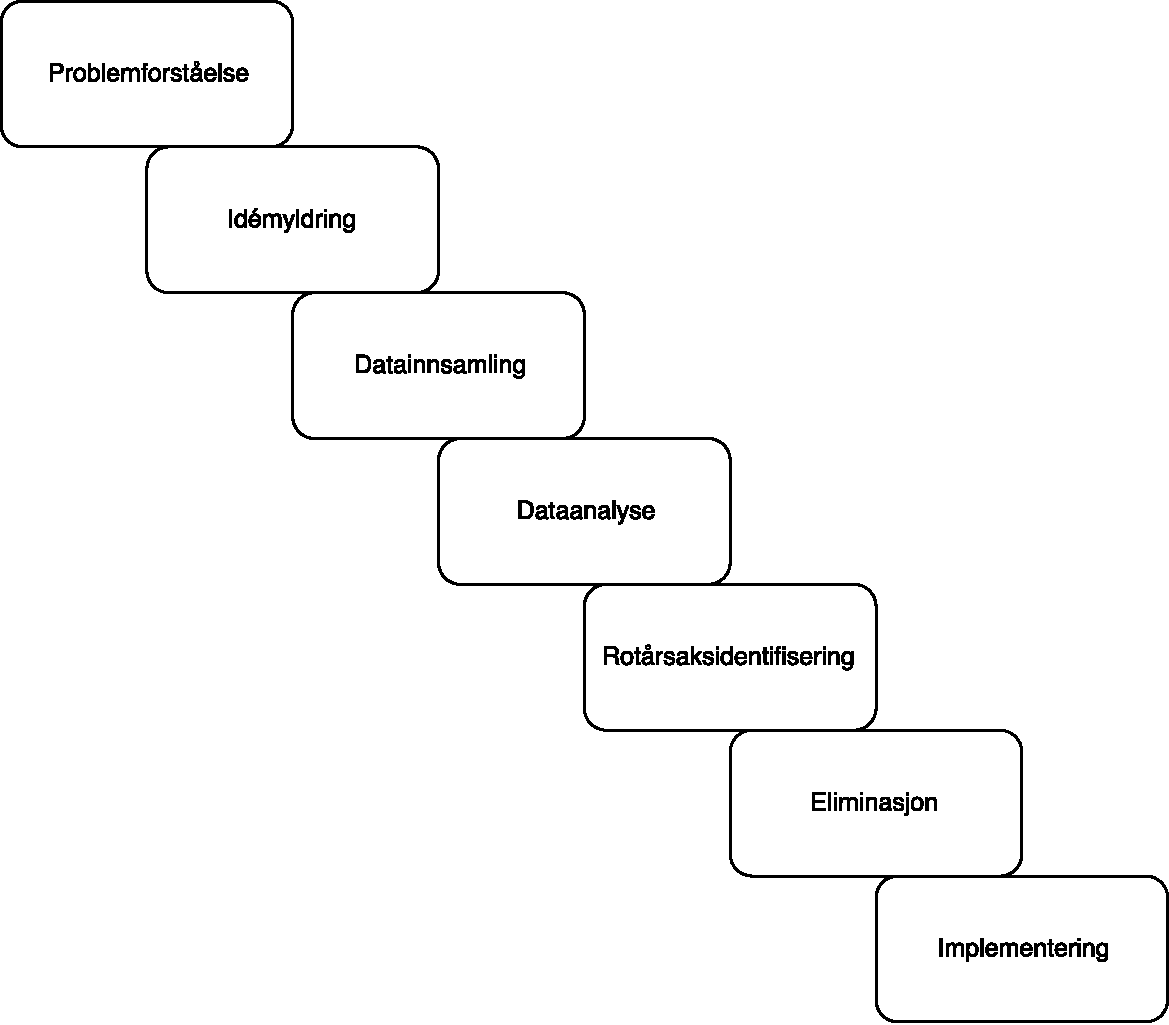
\includegraphics[scale=0.6]{prosess}
    \label{fig:prosess}
    \caption[Rotårsaksanalyseprosessen]{Rotårsaksanalyseprosessen definert av Andersen og Fagerli}
\end{figure}